%!TEX program = xelatex

\documentclass[a4paper, openany, oneside]{memoir}
\usepackage[no-math]{fontspec}
\usepackage{pgfplots}
\pgfplotsset{compat=newest}
\usepackage{commath}
\usepackage{mathtools}
\usepackage{amssymb}
\usepackage{amsthm}
\usepackage{booktabs}
\usepackage{mathtools}
\usepackage{xcolor}
\usepackage[separate-uncertainty=true, per-mode=symbol]{siunitx}
\usepackage[noabbrev, capitalize]{cleveref}
\usepackage{listings}
\usepackage[american inductor, european resistor]{circuitikz}
\usepackage{amsmath}
\usepackage{amsfonts}
\usepackage{ifxetex}
\usepackage[dutch,english]{babel}
\usepackage[backend=bibtexu,texencoding=utf8,bibencoding=utf8,style=ieee,sortlocale=en_GB,language=auto]{biblatex}
\usepackage[strict,autostyle]{csquotes}
\usepackage{parskip}
\usepackage{import}
\usepackage{standalone}
\usepackage{hyperref}
%\usepackage[toc,title,titletoc]{appendix}

\ifxetex{} % Fonts laden in het geval dat je met Xetex compiled
    \usepackage{fontspec}
    \defaultfontfeatures{Ligatures=TeX} % To support LaTeX quoting style
    \setromanfont{Palatino Linotype} % Tover ergens in Font mapje in root.
    \setmonofont{Source Code Pro}
\else % Terug val in standaard pdflatex tool chain. Geen ondersteuning voor OTT fonts
    \usepackage[T1]{fontenc}
    \usepackage[utf8]{inputenc}
\fi
\newcommand{\references}[1]{\begin{flushright}{#1}\end{flushright}}
\renewcommand{\vec}[1]{\boldsymbol{\mathbf{#1}}}
\newcommand{\uvec}[1]{\boldsymbol{\hat{\vec{#1}}}}
\newcommand{\mat}[1]{\boldsymbol{\mathbf{#1}}}
\newcommand{\fasor}[1]{\boldsymbol{\tilde{\vec{#1}}}}
\newcommand{\cmplx}[0]{\mathrm{j}}
\renewcommand{\Re}[0]{\operatorname{Re}}
\newcommand{\Cov}{\operatorname{Cov}}
\newcommand{\Var}{\operatorname{Var}}
\newcommand{\proj}{\operatorname{proj}}
\newcommand{\Perp}{\operatorname{perp}}
\newcommand{\col}{\operatorname{col}}
\newcommand{\rect}{\operatorname{rect}}
\newcommand{\sinc}{\operatorname{sinc}}
\newcommand{\IT}{\operatorname{IT}}
\newcommand{\F}{\mathcal{F}}

\newtheorem{definition}{Definition}
\newtheorem{theorem}{Theorem}


\DeclareSIUnit{\voltampere}{VA} %apparent power
\DeclareSIUnit{\pii}{\ensuremath{\pi}}

\hypersetup{%setup hyperlinks
    colorlinks,
    citecolor=black,
    filecolor=black,
    linkcolor=black,
    urlcolor=black
}

% Example boxes
\usepackage{fancybox}
\usepackage{framed}
\usepackage{adjustbox}
\newenvironment{simpages}%
{\AtBeginEnvironment{itemize}{\parskip=0pt\parsep=0pt\partopsep=0pt}
\def\FrameCommand{\fboxsep=.5\FrameSep\shadowbox}\MakeFramed{\FrameRestore}}%
{\endMakeFramed}

% Impulse train
\DeclareFontFamily{U}{wncy}{}
\DeclareFontShape{U}{wncy}{m}{n}{<->wncyr10}{}
\DeclareSymbolFont{mcy}{U}{wncy}{m}{n}
\DeclareMathSymbol{\Sha}{\mathord}{mcy}{"58}
\addbibresource{../../../../includes/bibliography.bib}

\begin{document}

\section{Introduction}
The fundamental problem of detection is to discern noise from a signal. This problem can be formulated as a binary hypothesis test. Given a signal $x[n]$ a detector has to decide between the following two hypotheses:

\begin{align*}
	\begin{cases}
		\mathcal{H}_0 & x[n] = w[n] \\
		\mathcal{H}_1 & x[n] = w[n] + s[n]
	\end{cases}
\end{align*}

where $w[n]$ denotes a noise signal and $s[n]$ a signal different from noise. Under $\mathcal{H}_0$ the signal $x[n]$ contains only noise. Under $\mathcal{H}_1$ another signal besides noise is present in $x[n]$.

Besides this hypothesis test, the detector also has to deal with frequency bands: which frequency bands are occupied by some signal and which are unoccupied?

This chapter examines three detectors that can be used in combination with our reconstructor:

\begin{enumerate}
	\item Conventional energy detection;
	\item Energy detection adapted to the reconstruction method;  
	\item Covariance absolute value detection (CAV).
\end{enumerate}

% Many other detectors exist, some of them using \emph{prior information} about the signals to be detected. Although the use of prior information
% makes detection of signals at a very low signal to noise ratio possible, we eventually have chosen not to depend on this \emph{prior information}. The reason for this is twofold:
% \begin{enumerate}
% 	\item By not depending on \emph{prior information} the detector can be used in a variety of situations,
% 	effectively providing us with a ``general '' purpose detector.
% 	\item The methods listed above have a relatively low complexity and therefore need less care to be implemented
% 	in our testing platform.
% \end{enumerate}

% This chapter will continue with a description and comparison of the three detection methods.

\section{Energy detection}
Conventional energy detection is a detection method that measures the energy of a signal $x[n]$, $\Lambda$, during a certain period. By comparing this measured energy to a threshold $\gamma$ the detector decides whether the input signal $x[n]$ contains only noise or that another signal besides noise is present in $x[n]$:

\begin{align*}
	\begin{cases}
		\mathcal{H}_0 & \text{if } \Lambda < \gamma \\
		\mathcal{H}_1 & \text{if } \Lambda > \gamma
	\end{cases}
\end{align*}
 
Given $N$ samples of $x[n]$, the measure of energy, $\Lambda$, which is used as test statistic is given by 

\begin{align}\label{eq:test_ed}
	\Lambda &= \sum_{n=0}^{N-1} |x[n]|^2.
\end{align}

The threshold $\gamma$ depends on the expected noise power $\sigma_n^2$ and the desired false alarm probability $p_{fa}$: the probability that the detector decides that hypothesis 2 is true, while hypothesis 1 is the true hypothesis. The derivation of $\gamma$ (see Appendix ...) gives the following result

\begin{align*}
\gamma = \left[Q^{-1}(p_{fa})\sqrt{N} + N\right]2\sigma_n^2
\end{align*}

where $Q^{-1}$ denotes the the inverse tail probability function of the standard normal distribution and $p_{fa}$ is the desired false alarm probability.
Using a bandpass filter $H(f)$ one can filter the signal $x[n]$ such that it can be used to detect a signal in a particular frequency band. This whole process is depicted
in \cref{tkz:conv_ed}
\begin{figure}[H]
\centering
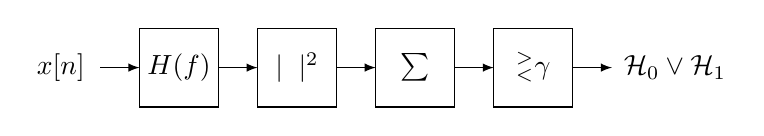
\begin{tikzpicture}

\node at (-6,2) {$x[n]$};
\node at (1.8,2) {$\mathcal{H}_0 \lor \mathcal{H}_1$};

\draw [>=latex, ->] (-5.5,2) -- (-5,2);
\draw (-5,2.5) rectangle (-4,1.5) node[pos=.5]{$H(f)$};

\draw [>=latex, ->] (-4,2) -- (-3.5,2);
\draw (-3.5,2.5) rectangle (-2.5,1.5) node[pos=.5]{$|\;\;|^2$};

\draw [>=latex, ->] (-2.5,2) -- (-2,2);
\draw (-2,2.5) rectangle (-1,1.5) node[pos=.5]{$\sum$};

\draw [>=latex, ->] (-1,2) -- (-0.5,2); 
\draw (-0.5,2.5) rectangle (0.5,1.5) node[pos=.5]{$_<^ > \gamma$};

\draw [>=latex, ->] (0.5,2) -- (1,2);

\end{tikzpicture}
\caption{Conventional Energy Detector}\label{tkz:conv_ed}
\end{figure}

% As can be seen from  \cref{eq:test_ed} the test statistic used by the conventional energy detector does not take into account that the signal to be detected resides in a certain frequency band. Therefore it is necessary that the input signal $x[n]$ is filtered before $\Lambda$ is computed.

As can be noted from \cref{eq:test_ed} the test statistic depends on the signal itself, not on the autocorrelation which serves as input of our detector.
In the rest of this section, we will show how the test statistic can be modified
such that the autocorrelation function can be used to detect the presence of  a signal in a certain frequency band.

Let 
\begin{align*}
\Lambda' &= \frac{\Lambda}{N}\\
	&= \frac{\sum_{n=0}^{N-1} |x[n]|^2}{N},
\end{align*}
then $\Lambda'$ is an estimate of the average power $E\left[|x[n]|^2\right]$ of the signal $x$. We can use $\Lambda'$ as test statistic by using a modified threshold $\gamma' = \frac{\gamma}{N}$. By definition of the power spectral density we know that integral over the power spectral density equals the expected average power:

\begin{align}\label{eq:average_power_psd}
E\left[\left|x[n]\right|^2\right] = \frac{1}{2\pi} \int_{-\pi}^{\pi}\mathcal{P}_x(\omega) \text{d}\omega.
\end{align}
Furthermore, by the Wiener-Khinchin theorem we have that, if $x[n]$ is wide-sense stationary (as is assumed in the reconstructor),
\begin{align}\label{eq:wiener_psd}
	\mathcal{P}_x(\omega) = \sum_{n=-\infty}^{\infty} r_x[n] \exp [2\pi j\omega].
\end{align}
By combining \cref{eq:average_power_psd} and \cref{eq:wiener_psd} we can relate the autocorrelation function to the test statistic $\Lambda'$.
The test statistic $\Lambda'$, however, still does not allow for detection in a certain frequency band.

 Notice that if $x[n]=w[n]$, its autocorrelation function equals a delta function: $r_x[n] = \sigma_n^2\delta[n]$, with $\sigma_n^2$ the average noise power. 
 Therefore the power spectral density of $x[n]$, denoted by $\mathcal{P}(\omega)$ equals  
 \begin{align*}
 \mathcal{P}_x(\omega) = \sum_{n=-\infty}^{\infty}r_x[n]e^{-jn\omega} = \sigma_n^2.
 \end{align*} The power spectral density is constant. If we want to detect the presence of a signal in a certain frequency band $W$, we can make use of this characteristic. Let

 \begin{align*}
 \Lambda'' &= \int_W \mathcal{P}(\omega) \text{d}\omega
 \end{align*}
denote the test statistic to detect a signal in the frequency band W.
 If we would integrate the power spectral density of noise over $W$ we obtain an average power of  $\frac{W}{2\pi} \sigma_n^2$. Therefore if we are to use $\Lambda''$ as test statistic, we have to use the modified threshold $\gamma'' = \frac{W}{2\pi} \gamma'$.

\subsection{Noise variance}
As indicated, knowledge of the noise variance is necessary for the energy detector to work. In practical situations this noise variance may be estimated from a reference measurement in an empty frequency band. 

\subsection{Energy detection with knowledge of the reconstructor}
The energy detector as described in \cite{ariananda2012compressive} uses the power spectral density $\mathcal{P}_x(\omega)$ as test statistic. To determine the threshold $\gamma_{\omega}$ for each element, the signal $x[n]$ is assumed to contain purely additive gaussian white noise. The distribution of the elements of the power spectral density is then approximated as a normal distribution (see Appendix \textbf{TODO}).

By determining $\mu (\omega)$ and $\sigma^2 (\omega)$, a threshold for each frequency $\omega$ given a false alarm probability can be calculated as:

\begin{align*}
\gamma(\omega) &= Q^{-1}(p_{fa})\sigma (\omega) + \mu (\omega) 
\end{align*}

Let 
$\vec{\mu} \in \mathbb{R}^{(2L+1)N}$ and $\vec{\sigma} \in \mathbb{R}^{(2L+1)N}$ denote the vectors, where element $k$ contains $\mu(\omega)$ and $\sigma(\omega)$ respectively evaluated at frequency $\omega = \frac{2\pi k}{(2L+1)N}$.

Then 
\begin{align*}
\vec{\mu} = \mat{F}\mat{R}^{\dagger}E\left[\vec{r}_y\right]
\end{align*}
and
\begin{align*}
\vec{\sigma} = \mat{F}\mat{R}^{\dagger}\mat{C}_{r_y} \left(\mat{R_c}^{\dagger}\right)^{H}\mat{F}^H
\end{align*}
as derived in \cite{ariananda2012compressive}. $\mat{C}_{r_y}$ denotes the covariance matrix of $\vec{r}_y$ and is defined as
\begin{align*}
 E\left[\vec{r}_y\vec{r}_y^H\right] - E\left[\vec{r}_y\right]E\left[\vec{r}_y^H\right]
\end{align*}

In case that $x[n]$ contains white noise with variance $\sigma_n$, the elements of $\mat{C}_{r_y}$ are given by

% \begin{align*}
% \text{Cov}\left(r_{y_r,y_s}[t],r_{y_u,y_v}[w]) &= \sigma_n^4 \frac{r_{c_r,c_u}[0]r_{c_s,c_v}[0]}\delta[w-t]}{(K-|k|)}
% \end{align*}

where $K$ denotes the amount of samples used to estimate the cross correlations between $d$.

\section{Covariance absolute value method}
The covariance absolute value detection method as introduced does \emph{not} depend on the noise power. Its test statistic is based on the structure of the autocorrelation function $r_x[n]$.

Let $L$ samples of the signal $x[n]$ be collected in the vector $\vec{x} = \left[x[n], x[n+1], \ldots, x[n+L]\right]$. 
Furthermore let $\mat{C}_x = E\left[\left(\vec{x} - \mu \right)\left(\vec{x} - \mu \right)^H\right]$ denote the covariance of $\vec{x}$ with $\mu = E[\vec{x}]$.

In the case that $E\left[\vec{x}\right]=0$, like for noise or most communication signals, then $\mat{C}_x$ can be simplified to

\begin{align*}
\mat{C}_x &= E\left[\vec{x}\vec{x}^T\right] \\
&= \begin{bmatrix} 
E\left(x[n][n]\right) & E\left(x[n][n+1]\right) & \ldots & E\left(x[n][n+L-1]\right) \\
E\left(x[n+1][n]\right) & E\left(x[n+1][n+1]\right) & \ldots & E\left(x[n+1][n+L-1]\right) \\
\vdots & \vdots & \ddots & \vdots \\
E\left(x[n+L-1][n]\right) & E\left(x[n+L-1][n+1]\right) & \ldots & E\left(x[n+L-1][n+L-1]\right) \\
\end{bmatrix}.
\end{align*}
Under the assumption that $x[n]$ is a wide-sense stationary signal, we can simplify $\mat{C}_x$ even further:
\begin{align*}
\mat{C}_x &= E\left[\vec{x}\vec{x}^T\right] \\
&= \begin{bmatrix} 
r_x[0] & r_x[1] & \ldots & r_x[L-1] \\
r_x[1] & r_x[0] & \ldots & r_x[L-2] \\
\vdots & \vdots & \ddots & \vdots \\
r_x[L-1] & r_x[L-2] & \ldots & r_x[0] \\
\end{bmatrix}.
\end{align*}

As stated in section \textbf{verwijs}, the autocorrelation function of white noise is a delta function. This implies that if $x[n]$ is white noise with variance $\sigma_n^2$ then $\mat{C}_x = \sigma_n^2\mat{I}$.
If the signal $x[n]$ is not equal to noise, then its autocorrelation function is not equal to a delta function which results in $\mat{C}_x$ having non-zero off diagonal elements.

Covariance absolute value method detection uses a measure of this ``diagonality'' of $\mat{C}_x$ as test statistic $\Lambda$.
This measure $\Lambda$ is defined as
\begin{align*}
\Lambda &= \frac{\sum_{n=1}^{L} \sum_{m=1}^L \left|\mat{C}_{nm}\right|}{\sum_{k=1}^L |\mat{C}_{kk}}
\end{align*} 

In practice one estimates the matrix $\mat{C}_x$ by using a limited amount of samples $N$ to estimate $r_x[n]$. The threshold given a desired false alarm probability
$p_{fa}$ is derived in \textbf{cite} to be

\begin{align*}
\gamma &= \frac{(1+(L-1)\sqrt{\frac{2}{N\pi}}}{1-Q^{-1}(p_{fa})\sqrt{\frac{2}{N}}}
\end{align*} 



% \subimport{detection/preliminaries/}{preliminaries}
% \subimport{detection/main_analysis/}{main_analysis}
% \subimport{detection/algorithm/}{algorithm}
% \subimport{detection/proofs/}{proofs}
\end{document}
